\documentclass[a4paper, 12pt]{report}
\usepackage[UTF8]{ctex}
\usepackage{amsmath}
\usepackage{amssymb}
\usepackage{graphicx}
\usepackage{xeCJK}
\begin{document}
\title{遗传学}
\author{Chickie Hu}
\date{\today}
\maketitle
\tableofcontents
\chapter{奇妙概念}
\begin{enumerate}
    \item 外显率:显性杂合或隐形纯合时预期表型的比例
    \item 表现度:相同基因型间表达变化程度
    \item 相互作用 \begin{enumerate}
              \item 不完全显性\&部分显性:显性杂合表现介于两个纯合之间
              \item 共显性\&镶嵌显性:一对等位基因被同时表达 e.g.MN血型
              \item 致死基因
              \item 复等位基因
          \end{enumerate}
    \item 非等位基因作用 \begin{enumerate}
              \item 基因互作:两个基因共同影响一个表型,\[9:3:3:1\],出现两非亲本型
              \item 抑制基因:一个基因抑制另一个基因的表达,\[13:3\]
              \item 互补基因:两个基因共同影响一个表型,\[9:7\],缺一不可
              \item 上位效应:一个基因影响另一个基因的表达 \begin{enumerate}
                        \item 显性上位:显性基因影响隐性基因,\[12:3:1\]
                        \item 隐性上位:隐性基因影响显性基因,\[13:3\]
                    \end{enumerate}
              \item 叠加效应:多个基因共同影响一个表型,e.g.荠菜三角形蒴果,当多条通路都被阻断时才会消失
          \end{enumerate}
\end{enumerate}
\chapter{统计}
\section{二项式定理}

\section{$\chi^2$检验}
\[\chi^2 = \sum \dfrac{(O_i - E_i)^2}{E_i}\]
\section{贝叶斯定理}
定义\(P(A|B)\)为B条件下A的概率函数,则有\[P(AB)=P(A|B)\times P(B)=P(B|A)\times P(A)\]
变形可得\[P(A|B)=\dfrac{P(B|A)\times P(A)}{P(B)}\]
称作\textbf{贝叶斯定理}
\section{似然函数}
对于概率函数\(P(x|\theta)\),似然函数\(L(\theta|x)\)定义为在给定\(x\)的情况下,\(\theta\)的概率密度函数,类比于主元变换。显然有\[L(\theta|x) = P(x|\theta)\]
\chapter{连锁分析}
\section{性连锁遗传}
\subsection{性别决定}
\begin{enumerate}
    \item XX-XY(注:\textit{Homo sapiens}的Y染色体与X有同源区段,减数分裂会发生重组)
    \item ZZ-ZW:鸟类、鳞翅目昆虫、某些两栖类、爬行类
    \item XO:直翅目昆虫,雌性为XX,雄性为XO
\end{enumerate}
\subsection{连锁}
\begin{itemize}
    \item 伴性遗传:连锁在同配染色体上(X,Z等),遗传时下一代满足
          \[
              \begin{aligned}
                  P_n(\text{异配性别}) & =P_{n-1}(\text{同配性别})                                            \\
                  P_n(\text{同配性别}) & =\frac{1}{2}P_{n-1}(\text{异配性别})+\frac{1}{2}P_{n-1}(\text{同配性别}) \\
              \end{aligned}
          \]
          \begin{figure}[htbp]
              \centering
              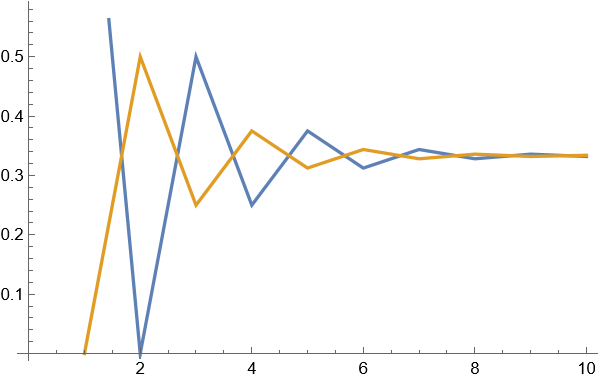
\includegraphics{image.png}
              \caption{伴性遗传基因频率变化}
              \label{伴性遗传}
          \end{figure}
    \item 限性遗传:连锁在异配染色体上
\end{itemize}
\subsection{遗传病}
\begin{itemize}
    \item 血友病
    \item Duchenne型肌营养不良
    \item 毛耳缘(Y连锁,限雄遗传)
\end{itemize}
\subsection{奇怪东西}
\begin{itemize}
    \item 雄果蝇、雌家蚕不会重组
    \item 果蝇的性别由性指数决定(X/A,1为雌,0.5为雄,中间间性),Y染色体只能让雄蝇可育
    \item 昆虫中常出现雌雄嵌合体现象:XX细胞丢失一条X形成XO细胞,发育成雄性性状
\end{itemize}
\section{剂量补偿}
\begin{itemize}
    \item 哺乳类:随机失活
    \item 有袋类:父本X染色体失活
    \item 果蝇:雄性X染色体超活性
    \item 秀丽隐杆线虫:两条X均低活性
\end{itemize}
\subsection{Lyon假说}
\begin{itemize}
    \item 1961年,Mary Lyon提出
    \item 随机失活:在胚胎发育早期,每个细胞中的一条X染色体被随机失活,失活的X染色体形成巴氏小体
    \item 杂合体形成\textbf{嵌合性状}
\end{itemize}
\section{连锁}
\subsection{遗传第三定律——连锁定律}
同一对染色体上基因联合在一起遗传的频率大于重新组合的频率\\
(交换发生在减一前期粗线期)
\subsection{计算}
重组值定义为
\[RF=\frac{\text{重组型数目}}{\text{总数目}}\]
注意,无论是二线、三线还是四线双交换,最大交换值均为0.5,更多次的交换同理;以及,二线双交换产生1PD,两种三线双交换各为1T,四线双交换产生1NPD。实际理论上双交换只有一半是重组型配子(但平时可能不会考虑)
\subsection{两点测交}
难以控制变量,不能测双交换,略
\subsection{三点测交}
杂合体与隐形纯和进行测交,最少的种类为双交换,且被交换的基因位于三个基因中央
计算重组值时需考虑双交换,视作两边的基因交换两次
\subsubsection{染色体干涉}
双交换的发生率通常比正常偏低,即\textbf{存在干涉},定义
\[
    \text{并发系数}C=\dfrac{\text{实际双交换率}}{\text{理论双交换率(单交换率乘积)}}
\]
同时有干涉值I=1-C;特殊情况会出现负干涉,即第一次交换后会促进第二次交换
\subsubsection{染色体单体干涉}
指4条染色单体参与多线交换的机会非随机性;理论情况应为二线:三线:四线=1:2:1,如果出现偏离即视为发生\textbf{染色体单体干涉}
如果四线双交换高于1/4,为正染色单体干涉;如果二线双交换升高,为负染色单体干涉

不出现干涉时,双交换平均重组率最大才是50\%
\subsubsection{校正}
重组值有最大值,但是\textbf{交换率}没有,应当在二者间建立一个函数关系。
由Poisson分布,有
\[
    P(X=k)=\frac{\lambda^k}{k!}e^{-\lambda}
\]
当平均交换数为\(\lambda\)时,交换k次的概率为P(k);又知道交换零次时,其对RF的贡献为0,但是它的概率为\[P(0)=e^{-\lambda}\]。
因此阻止RF达到最大值1/2的因素是\[e^{-\lambda}\],即
\[RF=\frac{1}{2}(1-e^{-\lambda})\]
从此式即可反解出平均交换率\(\lambda\)
\[
    \lambda=-\ln(1-2RF)
\]
\begin{figure}[htbp]
    \centering
    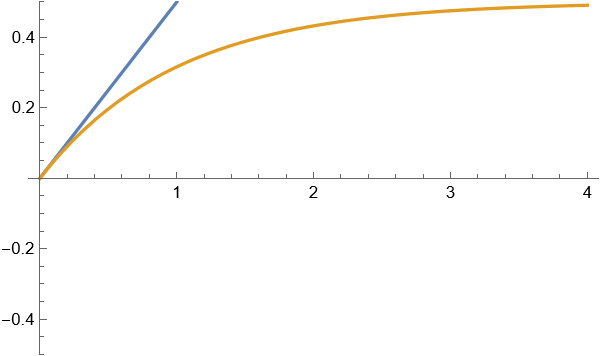
\includegraphics{交换率校正.png}
    \caption{重组率与校正后的交换率}
    \label{交换&重组}
\end{figure}
\subsubsection{四分子分析}
\paragraph{单基因}
计算其与着丝粒之间的交换率
\chapter{核外遗传}
\section{紫茉莉花斑叶}
叶绿体突变,母体遗传;在分裂过程中可能出现\textbf{细胞质分离和重组},导致出现镶嵌表型
\section{酵母小菌落}
因基因突变导致的生长速率缓慢,分为三种
\begin{enumerate}
    \item 核小菌落(aka. 分离型小菌落):核突变,为\(Pet^-\),遵循孟德尔遗传
    \item 中性小菌落:线粒体完全失去功能,同野生型杂交不会影响后代表型
    \item 抑制性小菌落:mtDNA部分缺失,在校正机制下进行修复,但是出现大规模缺失,重排,因而杂交后代仍然是抑制性小菌落(除非极少数情况下合子有丝分裂)
\end{enumerate}
\section{衣藻抗生素抗性}
由核外基因决定链霉素抗性,正反交结果不一样(交配型由核基因\textit{mt}决定,\(mt^+\)者保留细胞质基因)
\section{草履虫放毒性}
短时间结合只会交换细胞核基因,KK与kk相互交换,生成Kk;但是长时间交换会形成细胞质桥交换胞质,卡巴粒得以传递。
但Kk的放毒者并不稳定,自交后会出现基因分离,kk的后代无法维持卡巴粒,会逐渐消失
\section{果蝇感染性遗传}
部分果蝇对二氧化碳极度敏感,由称作\(\sigma\)的病毒样因子引起,可诱导雌蝇对二氧化碳敏感,通过卵子传递。
还有被称作“性比雌蝇”的现象,其后代性比严重失调,甚至不产生雄性后代;由一种类似于\(\sigma\)的螺旋体引起
\section{母体影响}
\subsection{短暂性母体影响}
欧洲麦蛾皮肤中含有色素,当母方无色时,后代表型不受影响,但当母方有色时,色素会残存在幼虫体内,致使基因型无色的幼虫短时间内也会有色
\subsection{长期性母体影响}
椎实螺左/右旋
\section{线粒体遗传}
\subsection{mtDNA结构}
\begin{itemize}
    \item 哺乳动物无内含子(酵母有)
    \item 半保留D环复制
    \item pol \(\gamma\) 为mtDNA复制酶, 为核基因
    \item 不受细胞周期调s控(听核基因的)
\end{itemize}
\subsection{蛋白合成}
\begin{itemize}
    \item 没有帽子
    \item 超摆动法则:第三位任意
    \item 存在特殊密码子,例如UGA为色氨酸
\end{itemize}
\subsection{核基因辅助}
核糖体蛋白、氨酰tRNA合成酶、聚合酶,结构蛋白,多数呼吸链复合体亚基
\subsection{线粒体病}
\begin{itemize}
    \item Leber遗传性视神经病:线粒体呼吸链复合物异常
    \item MERRF综合征(肌阵挛性癫痫及粗糙红纤维):线粒体tRNA突变
\end{itemize}
\section{叶绿体遗传}
\subsection{cpDNA结构}
\begin{itemize}
    \item 大约120-160kb
    \item 两个不称的反向重复序列,隔开为大单拷贝序列LSC和小单拷贝序列SSC
    \item 不含m5C
    \item 一个cp通常含有一至几十个cpDNA
    \item 编码Rubisco大亚基
\end{itemize}
\subsection{分类}
\begin{enumerate}
    \item 不含反向重复序列
    \item 有大的反向重复序列
    \item 多个IR串联重复
\end{enumerate}
\section{线粒体、叶绿体起源}
内共生学说;叶绿体来自蓝藻,线粒体来自好氧细菌;演化过程中向细胞核DNA转移,同时发生基因顺序改变
\section{植物雄性不育}
\subsection{核不育型}
较少,很容易被淘汰,例如光敏核不育水稻,多数含一对隐性基因ms
\subsection{质-核不育型}
细胞质不育基因S+育性恢复基因基因Rf,只有S+rf/rf才会不育
\subsubsection{三系法杂交}
\begin{itemize}
    \item 恢复系:N+Rf/Rf
    \item 保持系:N+rf/rf
    \item 不育系:S+rf/rf
\end{itemize}
\chapter{数量性状}
\section{连续性状}
\subsection{多基因假说}
连续性状由多个基因(称为微效基因)控制,完全杂合子自交后代服从正态分布

微效基因之间效应相加且相等,一般不存在显隐性关系(但可能存在增效和减效);对环境敏感,因而个体间差距较大,难以辨识每一个单独基因表型
\section{阈性状}
阈性状由多个基因控制,但只有在达到一定阈值时才表现出来,否则表现为正常表型
\section{统计学分析}
\subsection{QTL定位}
QTL即数量性状基因座,通过连锁分析,以通过周边的遗传位点分析QTL的位置。通常与数量性状有高相关性的有极大可能与QTL连锁
\subsection{LOD 最大优势计分法}
定义原假设\(H_0\):两个基因座之间没有QTL;备择假设\(H_1\):两个基因座之间有QTL。
在\(H_0\)假设下,可以计算出完全不连锁情况下的发生概率\(L_0\);而在\(H_1\)假设下,通过给定不同的\(\theta\)值(此处指交换率),可以计算出不同的发生概率\(L_1\)。
通过计算\(\mathrm{LOD} = \log{\dfrac{L_1}{L_0}}\),可以得到一个似然比(取最大的),它反映了统计结果对连锁与不连锁的不同支持率之比,从而判断是否接受原假设。通常在\(\mathrm{LOD} > 3\)时接受备择假设。
\section{数量性状遗传率}
\subsection{一切的基础——方差可加性}
从方差的定义,我们可以得到\[\sigma^2 = \dfrac{\sum(x_i-\bar{x})^2}{df}\]
而对于数量性状,我们可以将其分解为平均值和随机偏移值,即\[x_i=\bar{x}+P\]
将P称作表型值,且可进一步分解为基因型值和环境值,即\[P=G+E\]
由此我们可以得到\[\sigma^2 = \sigma^2_G + \sigma^2_E\]
这意味着两种\textbf{不相干}的因素所带来的方差可以被完全分离,即存在\textbf{方差可加性}。
\subsection{构成}
\begin{enumerate}
    \item 累加效应A:每个基因独立、相等的效应;可遗传
    \item 显性离差D:等位基因间的相互作用,可遗传但不可固定,且\(\sum D=0\)
    \item 互作离差I:\textbf{非等位基因}间的相互作用,较复杂,通常置于环境值中讨论
\end{enumerate}
因此,\(\sigma^2 = \sigma^2_A + \sigma^2_D + \sigma^2_I + \sigma^2_E\),也记作\(V_P = V_A + V_D + V_I + V_E\)。
其中\(V_P\)为表型方差,\(V_A\)为育种值方差或加性方差,\(V_D\)为显性离差方差,\(V_I\)为互作离差方差,\(V_E\)为环境方差。
\subsection{遗传率}
\begin{enumerate}
    \item 广义遗传率\(H^2\):\(H^2 = \dfrac{V_G}{V_P}\)
    \item 狭义遗传率\(h^2\):\(h^2 = \dfrac{V_A}{V_P}\)
\end{enumerate}
\subsubsection{遗传率的估计}
假设有一对等位基因Aa,隐形纯合与显性纯和杂交,得到\(F_2\)代,可列出以下数据
\begin{center}
    \begin{tabular}{ccccc}
        基因型 & 基因型值   & 频率      & \(fx\)      & \(fx^2\)               \\
        \hline
        AA  & \(a\)  & \(1/4\) & \(1/4a\)    & \(\dfrac{1}{4}a^2\)    \\
        Aa  & \(d\)  & \(2/4\) & \(2/4d\)    & \(\dfrac{2}{4}d^2\)    \\
        aa  & \(-a\) & \(1/2\) & \(1/4(-a)\) & \(\dfrac{1}{4}(-a)^2\) \\
    \end{tabular}
\end{center}
因此,基因型值平均值\[\mu=\dfrac{1}{4}a+\dfrac{2}{4}d+\dfrac{1}{4}(-a)=\dfrac{1}{2}d\]
方差
\[
    \begin{aligned}
        \sigma_G^2            & =\dfrac{\sum f(x-\mu)^2}{\sum f}                    \\
                              & =\dfrac{\sum fx^2-2\sum fx\mu+\sum f\mu^2}{\sum f}  \\
                              & =\dfrac{\sum fx^2-2\sum f\mu^2+\sum f\mu^2}{\sum f} \\
                              & =\dfrac{\sum fx^2-\sum f\mu^2}{\sum f}              \\
                              & =\dfrac{\sum fx^2-(\sum fx)^2/\sum f}{\sum f}       \\
        \because \sum f       & =1                                                  \\
        \therefore \sigma_G^2 & =\sum fx^2-\mu^2                                    \\
                              & =\sum fx^2-(\sum fx)^2                              \\
                              & =\dfrac12a^2+\dfrac14d^2                            \\
    \end{aligned}
\]

由于方差可加性,在存在n对互不干扰的基因时,有\[\sigma_G^2=\sum_{1}^{n}\dfrac{1}{2}a^2+\sum_{1}^{n}\dfrac{1}{4}d^2\]
记作\(V_G=\dfrac{1}{2}A+\dfrac{1}{4}D\)。
但是,\(V_{(P(F2))}=V_G+V_E=\dfrac{1}{2}A+\dfrac{1}{4}D+V_E\)。
所以首先将\(V_E\)剥离

注意到P1与P2的基因型都是确定的纯合子,因此\(V_G=0\),即可有
\[V_E=\dfrac{1}{2}(V_{P1}+V_{P2})\]
又由于F1代也为固定的杂合子,也可写作
\[V_E=\dfrac{1}{3}(V_{P1}+V_{P2}+V_{F1})\]

因此,可以推得
\[
    \begin{aligned}
        H^2 & =\dfrac{V_{F2}-V_E}{V_F2}                           \\
            & =\dfrac{V_{F2}-\dfrac{1}{2}(V_{P1}+V_{P2})}{V_{F2}} \\
    \end{aligned}
\]

对于\(h^2\),只需要\(V_A\),因此需要分离出\(V_D\),故需要引入两次测交后代B1,B2

对于B1,有
\begin{center}
    \begin{tabular}{ccccc}
        基因型 & 基因型值  & 频率      & \(fx\)   & \(fx^2\)   \\
        \hline
        AA  & \(a\) & \(1/2\) & \(1/2a\) & \(1/2a^2\) \\
        Aa  & \(d\) & \(1/2\) & \(1/2d\) & \(1/2d^2\) \\
    \end{tabular}
\end{center}
\[
    V_{B1}=\sum fx^2-\dfrac{(\sum fx)^2}{\sum f}=\dfrac{1}{4}a^2-\dfrac{1}{2}ad-\dfrac{1}{4}d^2
\]

对于B2
\begin{center}
    \begin{tabular}{ccccc}
        基因型 & 基因型值   & 频率      & \(fx\)      & \(fx^2\)      \\
        \hline
        aa  & \(-a\) & \(1/2\) & \(1/2(-a)\) & \(1/2(-a)^2\) \\
        Aa  & \(d\)  & \(1/2\) & \(1/2d\)    & \(1/2d^2\)    \\
    \end{tabular}
\end{center}
\[
    V_{B1}=\sum fx^2-\dfrac{(\sum fx)^2}{\sum f}=\dfrac{1}{4}a^2+\dfrac{1}{2}ad-\dfrac{1}{4}d^2
\]

因此,\(V_{B1}+V_{B2}=\dfrac{1}{2}a^2+\dfrac{1}{2}d^2=\dfrac{1}{2}V_A+\dfrac{1}{2}V_D\)。
又由于\(V_{F2}=\dfrac{1}{2}V_A+\dfrac{1}{4}V_D\),所以
\[
    \dfrac{1}{2}V_A=2V_{F2}-(V_{B1}+V_{B2})\\
\]
从而
\[
    \begin{aligned}
        h^2 & =\dfrac{\dfrac{1}{2}V_A}{\dfrac{1}{2}V_A+\dfrac{1}{4}V_D+V_E} \\
            & =\dfrac{2V_{F2}-(V_{B1}+V_{B2})}{V_{F2}}                      \\
    \end{aligned}
\]
\section{近亲繁殖}
\subsection{亲缘系数}
亲缘系数\(R\)定义为两个个体之间的亲缘关系,即两个个体共享的基因比例。对于同源个体,\(R=1\);对于无关个体,\(R=0\)。显然,每传一代,\(F\)减半。
因此,使用通径环进行计算。
\begin{figure}
    \centering
    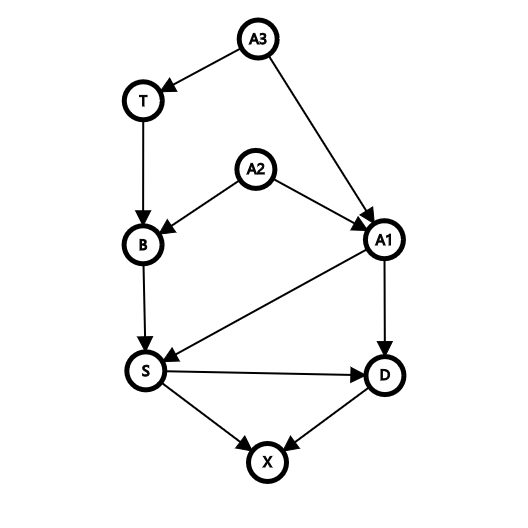
\includegraphics[width=1\textwidth]{近交图.png}
    \caption{通径图}
    \label{近交图}
\end{figure}
如图,对于B和A1个体,存在两个公共祖先A2和A3,存在通径B-T-A3-A1和B-A2-A1,因此\(R=(\frac{1}{2})^3+(\frac{1}{2})^2=\frac{3}{8}\)
\subsection{近交系数}
近交系数定义为获得一对遗传等同的基因的比例,对于常见的二倍体,每一个等位基因的传代都是\(\frac{1}{2}\)的概率,因此总体上计算同亲缘系数;综合两个等位基因的话,则有
\[F=\frac{1}{2}R\]
\textbf{但是},这仅限于二倍体,对于非标准情况还需要从定义出发进行计算。
\section{杂种优势}
杂种活力超过双亲中间值即可认定为有杂种优势,常见于种间杂种,例如骡
\subsection{杂种优势的来源}
一般有两种看法
\begin{enumerate}
    \item 显性说:近亲繁殖的不良效应和衰退是由杂合态基因分离,纯化导致,因此杂种能够综合双亲的优势基因。但也有不足
          \begin{enumerate}
              \item 理论上应当能够找到所有基因都是显性的纯合子,呈现F1代的表型
              \item 显性表型和隐形表型应是\((\frac{1}{4}+\frac{3}{4})^n\)的展开,为\textbf{偏态分布},但实际上更接近正态分布
          \end{enumerate}
    \item 超显性说:认为基因处在杂合态时的表现优于两个纯和态,并进一步认为复等位基因时靠每个等位基因作用差距来排序;但该理论完全否定了显性基因的作用
\end{enumerate}
\chapter{真核生物遗传分析}
\section{悖论}
\begin{itemize}
    \item C值悖论:基因组大小与进化程度不成关系
    \item N值悖论:基因数目与进化程度不成关系
\end{itemize}
\section{基因转变}
孢子囊内出现异常分离比,由基因转变为其对应的等位基因导致,分为
\begin{itemize}
    \item 染色单体转变:减数分裂一个产物转换,变为6:2
    \item 半染色单体转变:减数分裂半个产物转换,变为5:3;或两个半产物转换,变为4:4
\end{itemize}
切除修复造成。另,修复后表现跟交换一样,因此会出现并发系数>1
\section{体细胞交换}
\subsection{体细胞交换\&单倍体化}
以构巢曲霉为例,单倍体分生孢子会少量结合形成二倍体\textbf{异核体},含两个核,又有部分融合形成\textbf{合核体},更稳定,但也会分离成为\textbf{体细胞分离子},即\textbf{单倍体化}。

分离过程中产生一个三体和一个单体,三体常丢失一根染色体而恢复二倍体;单体常进一步丢失其他染色体成为单倍体,导致隐形表型出现,故称作分离。还有另外一种途径——构巢曲霉体细胞可以发生染色体交换(aka.有丝分裂交换)。这可以使杂合二倍体纯化为纯和二倍体,从而表现隐性性状
\subsection{有丝分裂交换}
在不进行有性生殖物种中可用于基因定位。例如abcd/++++,有丝分裂时实际为abcd/abcd/++++/++++,但是在有丝分裂交换后,可能会出现abc+/abcd/+++d/++++,分离后为abc+/++++(隐性基因表现),abcd/+++d或者abc+/+++d,abcd/++++,从而可以通过分离后的表型判断基因的位置。

这种连锁基因重组的方式又被称作准性生殖,但是不规律,不协调,以这种方式测量的cm值不准确
\section{基因消除\&染色体消减}
既然不用,直接丢掉,典型的如线虫,只有生殖系干细胞保留全套染色体。
高等植物中不存在该类现象,因而保留全能性。
\section{基因扩增}
例如爪蟾卵母细胞rDNA,滚环复制
\section{基因重排}
典型包括免疫球蛋白,锥虫表面糖蛋白
\subsection{酵母接合}
分为a和\(\alpha\)两种细胞,分别含有\(MATa\)和\(MAT\alpha\)基因,通过接合形成二倍体,再分裂形成单倍体

接合型的决定由两个沉默盒决定,\(HML\alpha\)和\(HMRa\),分别位于活跃盒左边和右边,由复制转座转移到活跃盒上表达,同时间只有一个盒子表达
沉默盒上游存在沉默子,同时缺少DNA酶\(\romannumeral1\)超敏位点,而恰好在活跃盒上游存在DNA酶\(\romannumeral1\)超敏位点,因此沉默盒沉默,活跃盒活跃
\chapter{细菌遗传}
\section{冷知识}
\begin{itemize}
    \item 细菌DNA依赖RNA形成紧密结构
    \item 不是所有细菌都是环状染色体,如放线菌,莱姆病螺旋体
    \item 细菌DNA含有甲基化酶,可以修饰DNA,防止受到限制性内切酶的攻击
\end{itemize}
\section{接合}
F因子转移,通过准性生殖产生重组后代,从\(F^+\)到\(F^-\),5'端先进;一般不足以让染色体进入,因此重组频率低,因此\(F^+\)称作Lfr低频重组

与此相对的是Hfr高频重组品系,F因子被整合在了染色体上,因此染色体会随着F因子转移,重组率高

接合时\(F^-\)得到的只是F因子一部分,因此接合后一般仍为\(F^-\),只形成不稳定的部分二倍体。且二倍体的交换必须是偶数次(否则形成开环),单向重组,重组子只有一种类型,另一半被抛弃
\subsection{中断杂交}
基因从Hfr转出时遵循一定的顺序,即在染色体上的排列顺序;可根据转移接合时间作图,单位为\textbf{分钟}而不是厘摩。

不同基因有其最大的转移频率,一般离起点越远越小
\subsection{重组作图}
首先得先筛选,确认某表型不出现不是因为不转移而是没重组。
例如\(lac-ade\),已知\(lac\)先于\(ade\)进入,那么,\(lac^+ade^+\)一定是在两侧进行的交换,而\(Lac^-ade^+\)则必定在两基因间发生重组,
但\(lac^+ade^-\)则单纯可能是还没进去,不用考虑,反而需要使用缺乏腺嘌呤的培养基筛选掉。

最后的重组率应该等于
\[
    RF=\dfrac{lac^-ade^+}{lac^+ade^++lac^-ade^+}
\]
\section{性导}
Hfr的F因子在剪切时带上了染色体的部分基因,形成F'因子,转移后形成稳定,可传代的部分二倍体。可见,F因子的存在与其“性别“有关,而F'因子又能形成稳定二倍体,因此称作性导
\section{转化}
细菌接受外来DNA分子并将其整合进自己的基因组,通过特定区域的临时性通道进入,外加感受态因子辅助

仅在对数期具备感受能力,称为\textbf{感受态细胞}
\subsection{转化作图}
基本原理同重组作图,略。

需注意如何判断连锁,在DNA低浓度时,转化频率与浓度成正比,若是不连锁(分别来自两个片段),则在DNA浓度下降时共转导频率降速远高于单基因转导频率,但连锁则不影响
\section{转导}
以病毒做载体转移基因,典型如最早发现的沙门氏菌LT22菌株和其P22噬菌体
\subsection{普遍性转导}
噬菌体在组装时完全随机的携带寄主的部分染色体,任意基因均可转入,但容量有限,频率低,约为\(10^{-5}\)

连锁特别紧密的可以发生共转导,因此可用于转导作图(注意,在三分子作图时,哪怕是基因间没有发生重组,也是双交换,如果只转入了两侧的基因,那得是四交换)

在计算图距时,有
\[
    d=L(1-\sqrt[3]{x})
\]

同时还会出现一类被称作流产转导的小菌落,基因没能重组进染色体,只能停留在细胞质中,当传家宝,而其他没得到DNA的只能靠残留的酶苟活
\subsection{局限性转导}
例如\(\lambda\)噬菌体,只能重组在特异位点\(attB\)上,两边为\(lac\)和\(bio\),因此特异转导这两个基因

实际\(\lambda\)噬菌体释放时,\(attB\)位点为杂种(一半来自细菌,一半来自噬菌体);如此,重组有两种情况:一种只重组\(lac\)基因,而另一种通过杂合\(attB\)整合进染色体(意思是染色体上必须还有一个\(\lambda\))。
对于后者,这种转导子溶菌产物正常的\(\lambda\)会辅助缺陷型的组装,提高转导频率,因此称作\textbf{辅助噬菌体}
\chapter{病毒遗传分析}
\section{常见种类}
\begin{itemize}
    \item 类病毒:ssRNA
    \item T4:dsDNA
    \item 脊髓灰质病毒:ssRNA,线性染色体
    \item 口蹄疫FMDV:ssRNA,线性染色体
    \item 疱疹病毒:dsDNA,线性染色体
    \item 乙型肝炎HBV:dsDNA
\end{itemize}
\section{噬菌体}
烈性、温和;对于温和噬菌体,整合后称为原噬菌体,有两重要特性
\begin{itemize}
    \item 免疫性:产生一种阻遏蛋白,阻止自身和外来噬菌体复制,防止二次感染
    \item 可诱导性:每代万分之一概率自发裂解,产生大量噬菌体
\end{itemize}
\subsection{突变型}
\begin{itemize}
    \item 条件致死突变型
          \begin{itemize}
              \item 温度敏感突变
              \item 抑制因子敏感突变:部分密码子突变为终止密码子,可通过特殊tRNA校正,即无义抑制基因\(su^+\)\begin{itemize}
                        \item 琥珀突变 UAG
                        \item 赭石突变 UAA
                        \item 乳白突变 UGA
                    \end{itemize}
          \end{itemize}
    \item 噬菌斑形态突变
          \begin{itemize}
              \item 烈性噬菌体:清晰
              \item 温和噬菌体:混浊
          \end{itemize}
    \item 宿主范围突变:感染时吸附于细菌专一受体,受体种类决定了可感染菌种,决定了噬菌斑大小
\end{itemize}
\subsection{重组测验}
\subsubsection{T4}
进行双重感染,收集产生的噬菌体,使用特殊菌种(宿主范围限定)进行筛选,只有\(++\)才能生长,但是\(--\)实际也是重组型,需要被计算,所以
\[
    RF=\dfrac{++*2}{\text{噬菌斑总数}}
\]
\subsubsection{T2}
突变型\(r^-\)为快速溶菌,产生大的溶菌斑,突变型\(h……-\)能同时感染品系1和2,噬菌斑透明,否则会因不感染品系2而半透明。

杂交使用品系1,再在品系1,2混合培养基中筛选
\[
    RF=\dfrac{(h^+r^+)+{h^-r^-}}{\text{总噬菌斑}}
\]
\subsubsection{\(\lambda\)}
\(s\)为小噬菌斑,\(c\)为完全清亮噬菌斑,\(mi\)为微小噬菌斑
\subsubsection{notice}
噬菌体的重组发生在复制之后,因此可以从同一个细菌中得到亲本型和重组型。同时,重组的发生与时间直接挂钩,需要严格控制时间才能得到近似的遗传图

T2和T4虽然是线性染色体,但做出来的遗传图却是环状的,是因为特殊的\textbf{多联体}
\subsection{互补测试}
略
\subsubsection{基因内互补}
特殊情况下,发生在同一个顺反子内的突变也能互补,典型的如多亚基蛋白,一个活性位点突变,一个激活位点突变,但杂合起来也能用,e.g.沙门氏杆菌GAPDH,大肠杆菌/脉孢霉色氨酸合成酶,脉孢霉谷酰脱氢酶
\subsection{缺失作图}
基因发生缺失时,是不能在该区域发生重组的,因此可通过检验缺失突变和点突变之间重组型量来验证其是否在该缺失区域内。
如果出现少量零散噬菌斑,可能是回复突变
\subsection{原噬菌体}
切除时可能出现偏差,将部分基因替换为E.\textit{coli}的基因,对于\(\lambda\),一般带\(bio\)没事,而带\(gal\)通常会置换掉部分必须基因
\chapter{基因组学}
\section{人类基因组}
\begin{itemize}
    \item 基因\&相关系列
          \begin{itemize}
              \item 基因
                    \begin{itemize}
                        \item 假基因
                        \item 基因片段
                        \item 内含子
                    \end{itemize}
              \item 基因间序列
                    \begin{itemize}
                        \item 散在重复序列
                              \begin{itemize}
                                  \item LINE
                                  \item SINE
                                  \item LTR元件
                                  \item DNA转座子
                              \end{itemize}
                        \item 其它基因间序列
                              \begin{itemize}
                                  \item 微卫星
                                  \item 各种间隔区
                              \end{itemize}
                    \end{itemize}
          \end{itemize}
\end{itemize}
\section{基因组测序}
\subsection{策略}
\begin{itemize}
    \item 自上而下:建立连续叠连克隆群,对单个叠连群进行鸟枪法测序后拼接
    \item 自下而上:全基因鸟枪法,
\end{itemize}


\chapter{
  果蝇发育
 }
\begin{itemize}
    \item 母源基因:存储在卵细胞中的各种mRNA和蛋白,负责体轴的形成
    \item 分节基因:合子活性基因,受精后被激活,决定体节数目和极性
    \item 同源异形基因(\textit{Hox}基因):本质上是一系列转录因子,决定各体节的分化
    \item 间隔基因:促进同源异形基因的表达,突变会导致一些连续体节段的缺失
\end{itemize}
\end{document}